% Figure 1 of "When Should a Quantity Have Its Own Dimension?"
% Symmetric arrangement of electromagnetic quantities (after Suga, Parity 12(4), 1997, Fig. 1).
%
% Build:   pdflatex Figure_1.tex
%          then rasterize at 326 dpi, e.g.
%            pdftoppm -png -r 326 -singlefile Figure_1.pdf Figure_1     (Poppler)
%            rungs -q -sDEVICE=png16m -r326 -o Figure_1.png Figure_1.pdf (TeX Live's Ghostscript)
%
% Uses only core TikZ (no arrows.meta), so it also compiles with PGF 2.x.
% Coordinates are in pixels of the 326-dpi raster (y grows downward).
\documentclass[border=0pt]{standalone}
\usepackage{amsmath}
\usepackage{tikz}
% axis-aligned arrows with a straight-sided filled head
%   \arrR{x1}{x2}{y}  rightwards from x1 to x2      \arrL{x1}{x2}{y}  leftwards
%   \arrD{x}{y1}{y2}  downwards from y1 to y2       \arrU{x}{y1}{y2}  upwards
\newcommand\arrR[3]{\draw (#1,#3) -- (#2-18,#3);
  \fill (#2,#3) -- (#2-21,#3-7.7) -- (#2-21,#3+7.7) -- cycle;}
\newcommand\arrL[3]{\draw (#1,#3) -- (#2+18,#3);
  \fill (#2,#3) -- (#2+21,#3-7.7) -- (#2+21,#3+7.7) -- cycle;}
\newcommand\arrD[3]{\draw (#1,#2) -- (#1,#3-18);
  \fill (#1,#3) -- (#1-7.7,#3-21) -- (#1+7.7,#3-21) -- cycle;}
\newcommand\arrU[3]{\draw (#1,#2) -- (#1,#3+18);
  \fill (#1,#3) -- (#1-7.7,#3+21) -- (#1+7.7,#3+21) -- cycle;}
\begin{document}
\fontsize{11.3pt}{13.6pt}\selectfont
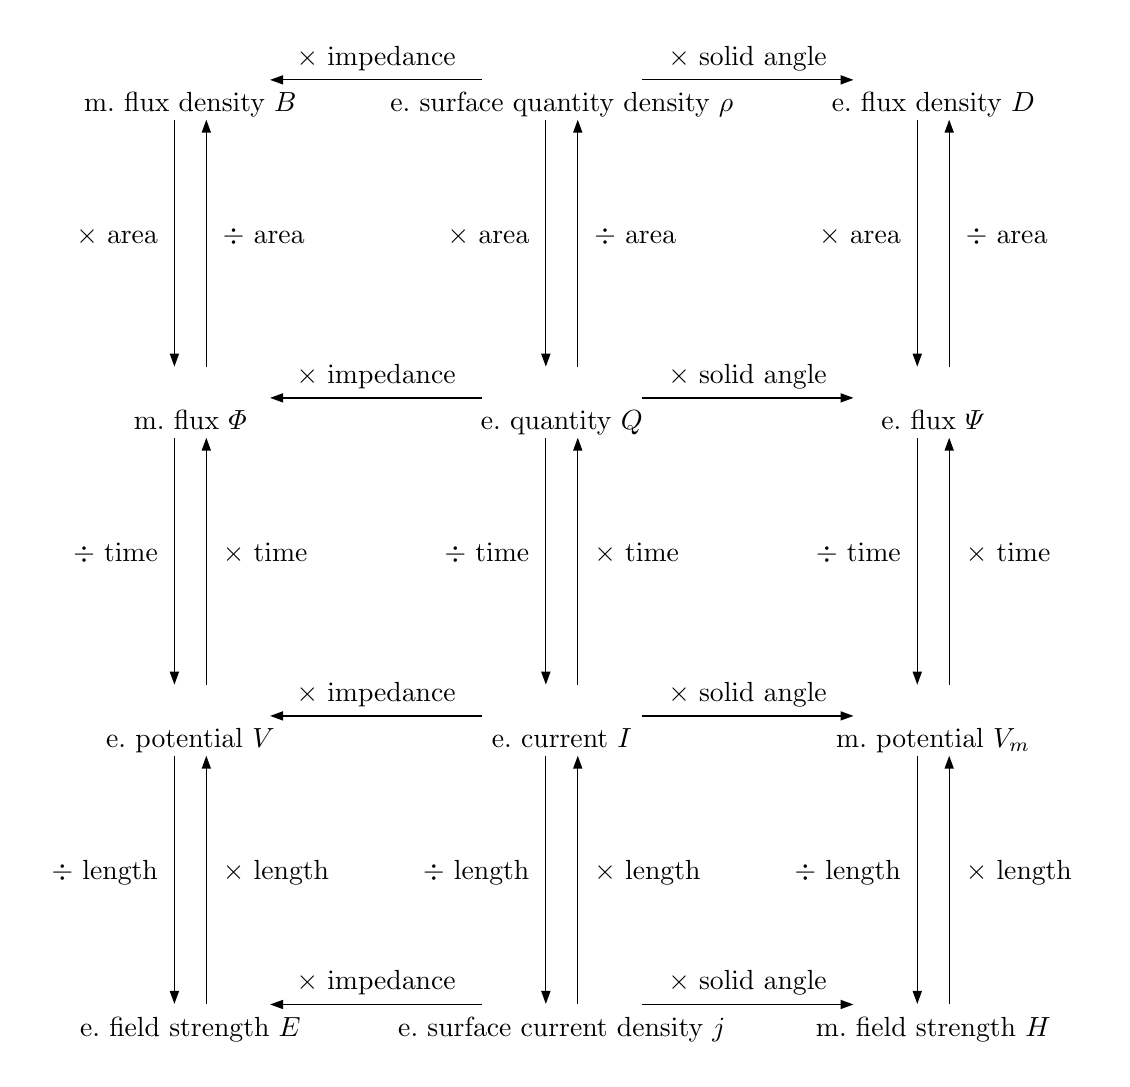
\begin{tikzpicture}[x=0.0077914cm, y=-0.0077914cm, line width=0.45pt,
    lab/.style={inner sep=0pt, anchor=base}]
  \useasboundingbox (-30,0) rectangle (1720,1680);
  % column centres and label baselines
  \def\xL{235} \def\xM{840} \def\xR{1445}
  \def\yA{137} \def\yB{655} \def\yC{1173} \def\yD{1643}
  % ---- entries -------------------------------------------------------
  \node[lab] at (\xL,\yA) {m.\ flux density $B$};
  \node[lab] at (\xM,\yA) {e.\ surface quantity density $\rho$};
  \node[lab] at (\xR,\yA) {e.\ flux density $D$};
  \node[lab] at (\xL,\yB) {m.\ flux $\varPhi$};
  \node[lab] at (\xM,\yB) {e.\ quantity $Q$};
  \node[lab] at (\xR,\yB) {e.\ flux $\varPsi$};
  \node[lab] at (\xL,\yC) {e.\ potential $V$};
  \node[lab] at (\xM,\yC) {e.\ current $I$};
  \node[lab] at (\xR,\yC) {m.\ potential $V_m$};
  \node[lab] at (\xL,\yD) {e.\ field strength $E$};
  \node[lab] at (\xM,\yD) {e.\ surface current density $j$};
  \node[lab] at (\xR,\yD) {m.\ field strength $H$};
  % ---- horizontal arrows: x impedance (leftwards), x solid angle (rightwards)
  \foreach \ya in {85,603,1121,1591}{
    \arrL{\xM-130}{\xL+130}{\ya}
    \arrR{\xM+130}{\xR-130}{\ya}
    \node[lab] at (537.5,\ya-24)  {$\times$ impedance};
    \node[lab] at (1142.5,\ya-24) {$\times$ solid angle};
  }
  % ---- vertical arrow pairs ------------------------------------------
  \foreach \x in {\xL,\xM,\xR}{
    \foreach \ytop/\ybot in {150/552, 668/1070, 1186/1590}{
      \arrD{\x-26}{\ytop}{\ybot}
      \arrU{\x+26}{\ybot}{\ytop}
    }
    \node[lab, anchor=base east] at (\x-52,352)  {$\times$ area};
    \node[lab, anchor=base west] at (\x+52,352)  {$\div$ area};
    \node[lab, anchor=base east] at (\x-52,870)  {$\div$ time};
    \node[lab, anchor=base west] at (\x+52,870)  {$\times$ time};
    \node[lab, anchor=base east] at (\x-52,1388) {$\div$ length};
    \node[lab, anchor=base west] at (\x+52,1388) {$\times$ length};
  }
\end{tikzpicture}
\end{document}
